\section{The Definite Integral} \label{S:4.3.DefiniteIntegral}

\vspace*{-14 pt}
\framebox{\hspace*{3 pt}
\parbox{\boxwidth}{\begin{goals}
\item How does increasing the number of subintervals affect the accuracy of the approximation generated by a Riemann sum?
\item What is the definition of the definite integral of a function $f$ over the interval $[a,b]$?
\item What does the definite integral measure exactly, and what are some of the key properties of the definite integral?
\end{goals}} \hspace*{3 pt}}

\subsection*{Introduction}

In Figure~\ref{F:4.2.NegF}, which is repeated below as Figure~\ref{F:4.3.IncreaseN}, we see visual evidence that increasing the number of rectangles in a Riemann sum improves the accuracy of the approximation of the net signed area that is bounded by the given function on the interval under consideration.
\begin{figure}[h]
\begin{center}
\scalebox{0.9}{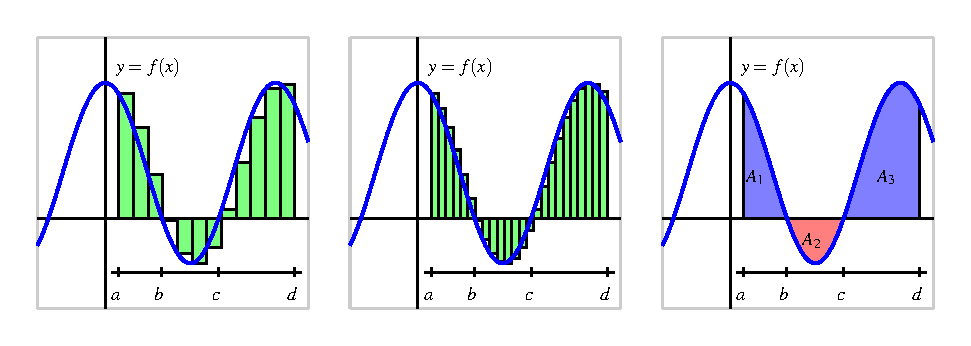
\includegraphics{figures/4_2_NegF.eps}}
\caption{At left and center, two left Riemann sums for a function $f$ that is sometimes negative; at right, the exact areas bounded by $f$ on the interval $[a,d]$.} \label{F:4.3.IncreaseN}
\end{center}
\end{figure}
We thus explore the natural idea of allowing the number of rectangles to increase without bound in an effort to compute the exact net signed area bounded by a function on an interval.  In addition, it is important to think about the differences among left, right, and middle Riemann sums and the different results they generate as the value of $n$ increases.  As we have done throughout our investigations with area, we begin with functions that are exclusively positive on the interval under consideration.

\begin{pa} \label{PA:4.3}
Consider the applet found at \href{http://gvsu.edu/s/a9}{\texttt{http://gvsu.edu/s/aw}}\footnote{Marc Renault, Shippensburg University, Geogebra Applets for Calclulus, \href{http://gvsu.edu/s/5p}{\texttt{http://gvsu.edu/s/5p}}.}.  There, you will initially see the situation shown in Figure~\ref{F:4.3.GGBApplet}.
\begin{figure}[h]
\begin{center}
\scalebox{0.4}{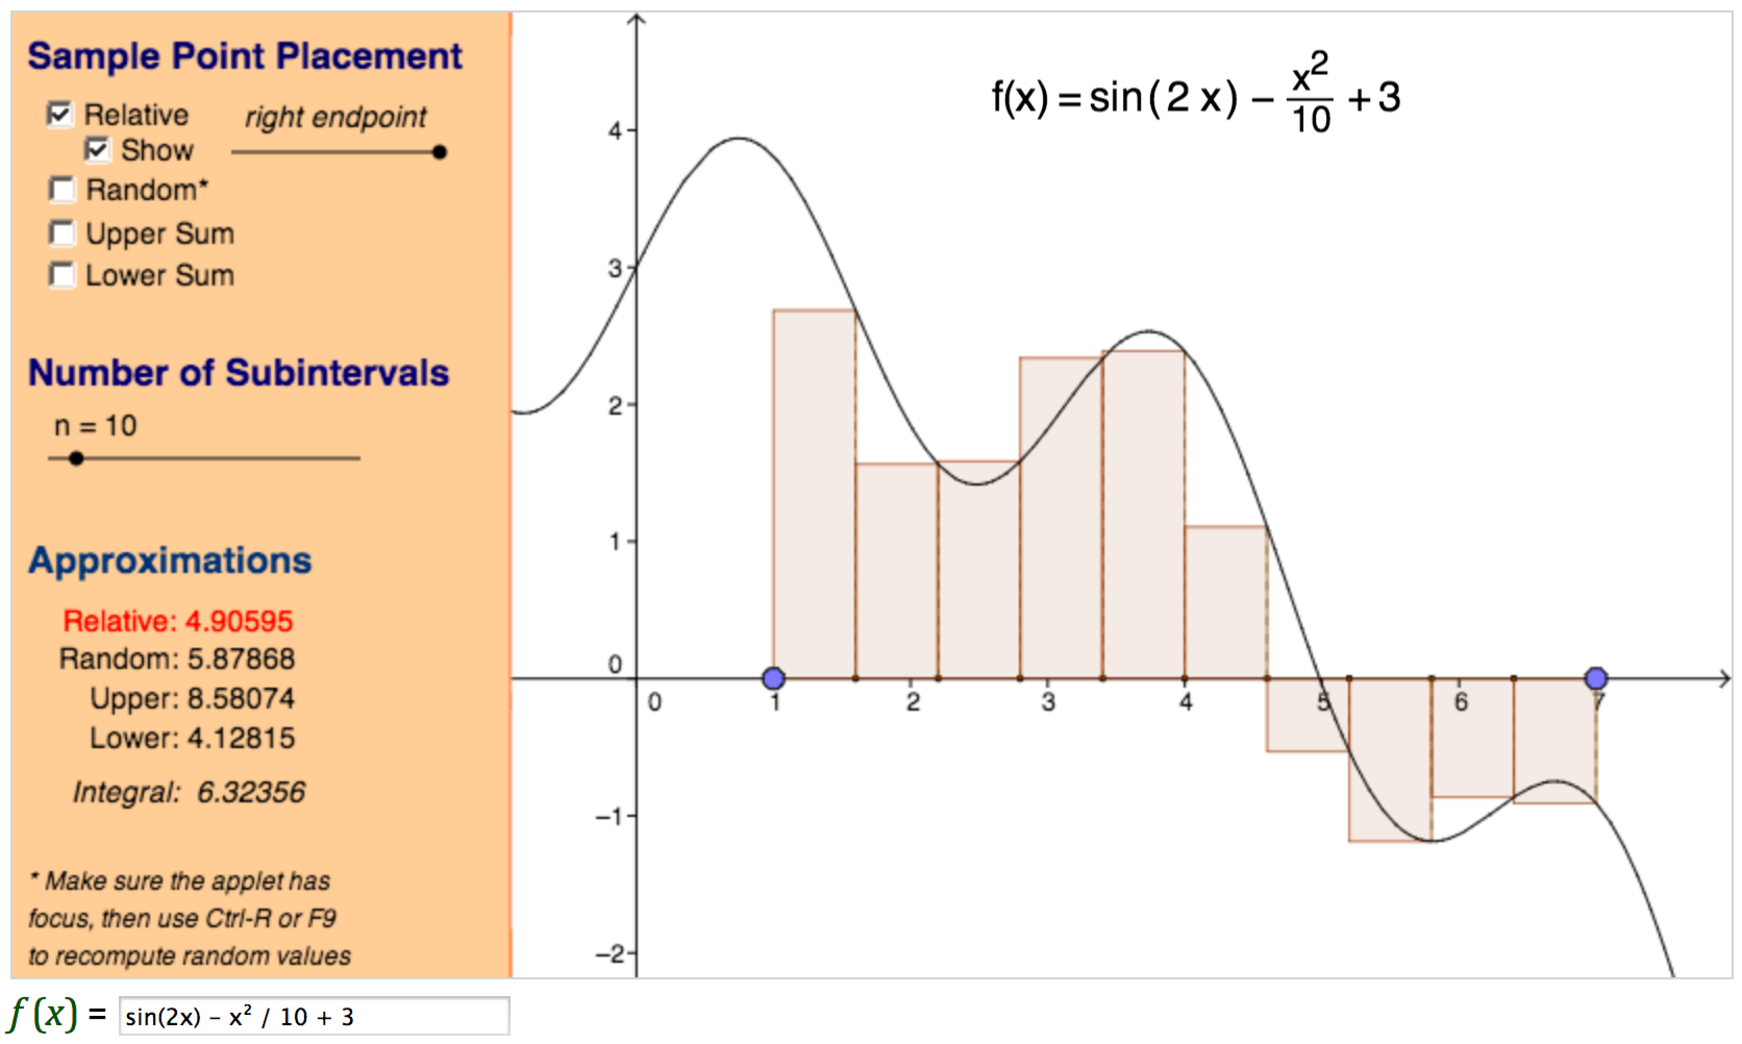
\includegraphics{figures/4_3_GGBApplet.pdf}}
\caption{A right Riemann sum with 10 subintervals for the function $f(x) = \sin(2x) - \frac{x^2}{10} + 3$ on the interval $[1,7]$.  The value of the sum is $R_{10} = 4.90595$.} \label{F:4.3.GGBApplet}
\end{center}
\end{figure}
Note that the value of the chosen Riemann sum is displayed next to the word ``relative,'' and that you can change the type of Riemann sum being computed by dragging the point on the slider bar below the phrase ``sample point placement.''

Explore to see how you can change the window in which the function is viewed, as well as the function itself.  You can set the minimum and maximum values of $x$ by clicking and dragging on the blue points that set the endpoints; you can change the function by typing a new formula in the ``f(x)'' window at the bottom; and you can adjust the overall window by ``panning and zooming'' by using the Shift key and the scrolling feature of your mouse.  More information on how to pan and zoom can be found at \href{http://gvsu.edu/s/Fl}{\texttt{http://gvsu.edu/s/Fl}}. 

Work accordingly to adjust the applet so that it uses a left Riemann sum with $n = 5$ subintervals for the function is $f(x) = 2x + 1$.  You should see the updated figure shown in Figure~\ref{F:4.3.GGBApplet2}.  Then, answer the following questions.
\begin{figure}[h]
\begin{center}
\scalebox{0.4}{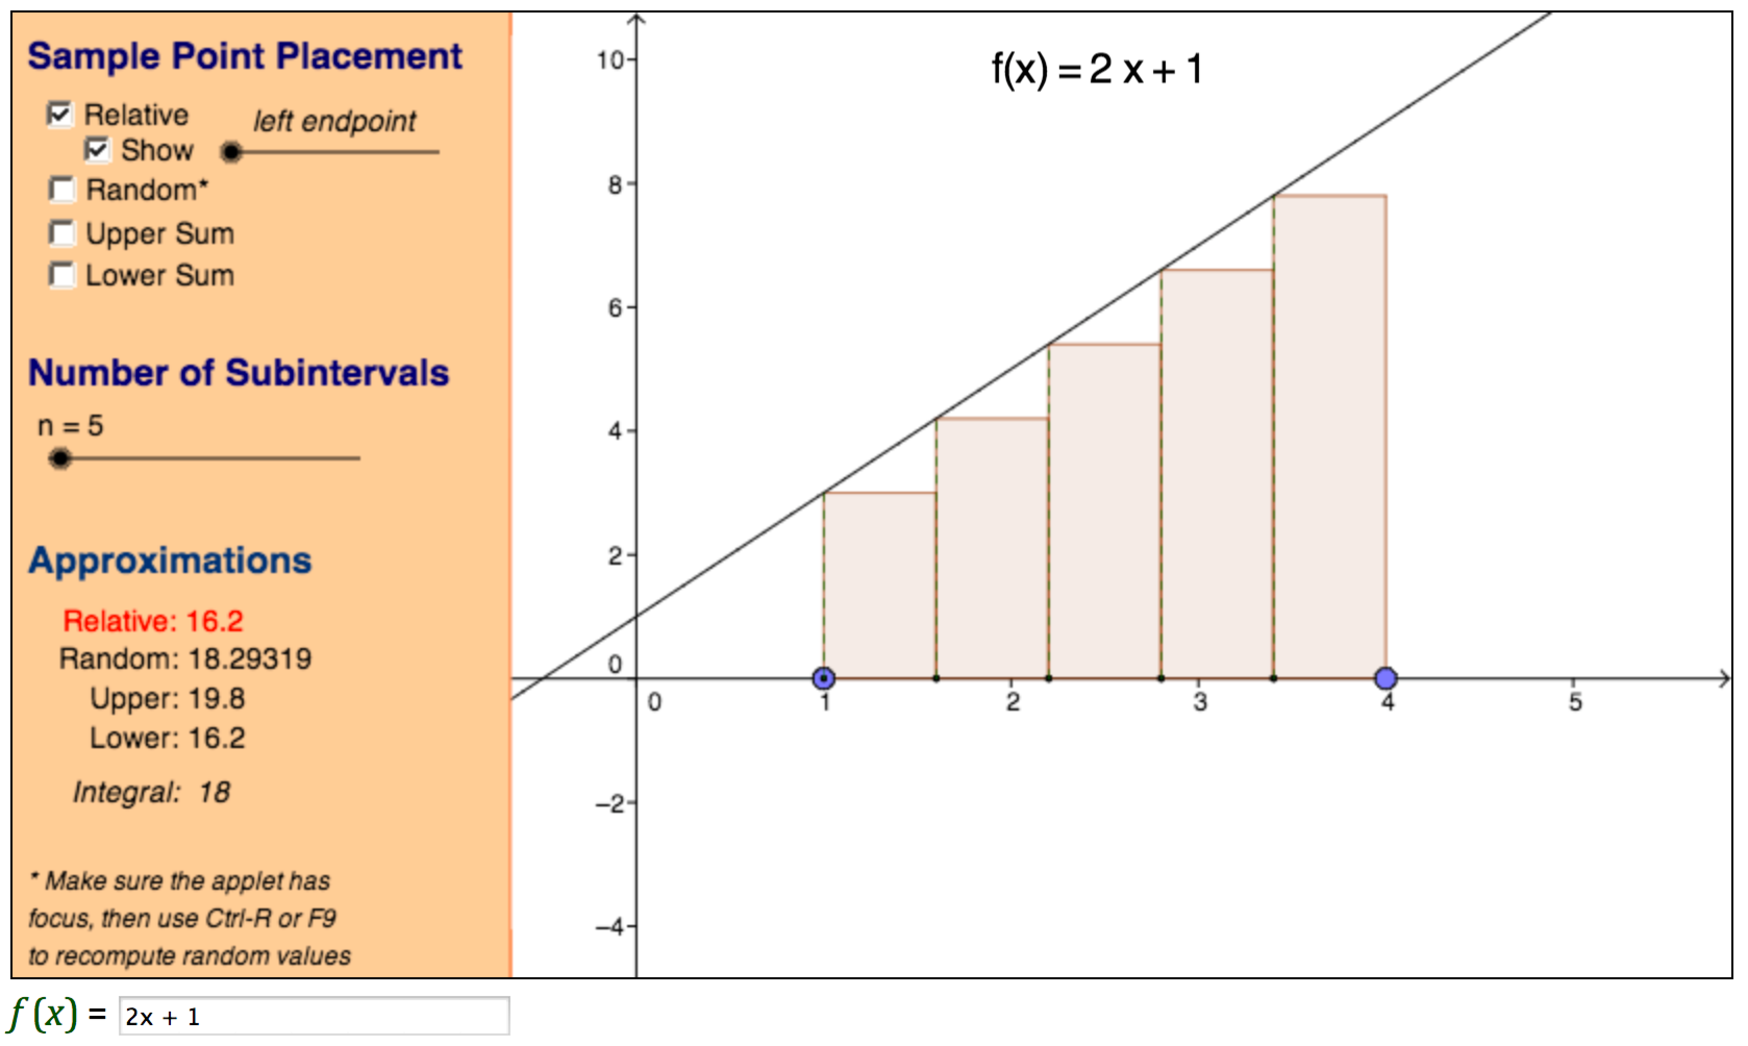
\includegraphics{figures/4_3_GGBApplet2.pdf}}
\caption{A left Riemann sum with 5 subintervals for the function $f(x) = 2x+1$ on the interval $[1,4]$.  The value of the sum is $L_5 = 16.2$.} \label{F:4.3.GGBApplet2}
\end{center}
\end{figure}
%Note that the value of the Riemann sum of our choice is displayed in the upper left corner of the window.  Further, by updating the value in the ``Intervals'' window and/or the ``Method'', we can see the different value of the Riemann sum that arises by clicking the ``Compute!'' button.
\ba
	\item Update the applet (and view window, as needed) so that the function being considered is $f(x) = 2x+1$ on $[1,4]$, as directed above.  For this function on this interval, compute $L_{n}$, $M_{n}$,  $R_{n}$ for $n = 5$, $n = 25$, and $n = 100$.  What appears to be the exact area bounded by $f(x) = 2x+1$ and the $x$-axis on $[1,4]$?
	\item Use basic geometry to determine the exact area bounded by $f(x) = 2x+1$ and the $x$-axis on $[1,4]$.
	\item Based on your work in (a) and (b), what do you observe occurs when we increase the number of subintervals used in the Riemann sum?
	\item Update the applet to consider the function $f(x) = x^2 + 1$ on the interval $[1,4]$ (note that you need to enter ``\texttt{x$\wedge$2 + 1}'' for the function formula).  Use the applet to compute $L_{n}$, $M_{n}$,  $R_{n}$ for $n = 5$, $n = 25$, and $n = 100$.  What do you conjecture is the exact area bounded by $f(x) = x^2+1$ and the $x$-axis on $[1,4]$?
	\item Why can we not compute the exact value of the area bounded by $f(x) = x^2+1$ and the $x$-axis on $[1,4]$ using a formula like we did in (b)?
\ea
\end{pa} 
\afterpa

\subsection*{The definition of the definite integral} \index{definite integral!definition}

In both examples in Preview Activity~\ref{PA:4.3}, we saw that as the number of rectangles got larger and larger, the values of $L_n$, $M_n$, and $R_n$ all grew closer and closer to the same value.  It turns out that this occurs for any continuous function on an interval $[a,b]$, and even more generally for a Riemann sum using any point $x_{i+1}^*$ in the interval $[x_i, x_{i+1}]$.  Said differently, as we let $n \to \infty$, it doesn't really matter where we choose to evaluate the function within a given subinterval, because
$$\lim_{n \to \infty} L_n = \lim_{n \to \infty} R_n = \lim_{n \to \infty} M_n = \lim_{n \to \infty} \sum_{i=1}^{n} f(x_i^*) \triangle x.$$  
That these limits always exist (and share the same value) for a continuous\footnote{It turns out that a function need not be continuous in order to have a definite integral.  For our purposes, we assume that the functions we consider are continuous on the interval(s) of interest.  It is straightforward to see that any function that is piecewise continuous on an interval of interest will also have a well-defined definite integral.} function $f$ allows us to make the following definition.
\begin{definition} \label{D:4.3.DefInt}
The \emph{definite integral} of a continuous function $f$ on the interval $[a,b]$, denoted $\ds \int_a^b f(x) \, dx$, is the real number given by
$$\int_a^b f(x) \, dx = \lim_{n \to \infty} \sum_{i=1}^{n} f(x_i^*) \triangle x,$$
where $\triangle x = \frac{b-a}{n}$, $x_i = a + i\triangle x$ (for $i = 0, \ldots, n$), and $x_i^*$ satisfies $x_{i-1} \le x_i^* \le x_i$ (for $i = 1, \ldots, n$).
\end{definition}
We call the symbol $\int$ the \emph{integral sign}\index{integral sign}, the values $a$ and $b$ the \emph{limits of integration}\index{limits of integration}, and the function $f$ the \emph{integrand}\index{integrand}.  The process of determining the real number $\int_a^b f(x) \, dx$ is called \emph{evaluating the definite integral}.  While we will come to understand that there are several different interpretations of the value of the definite integral, for now the most important is that $\int_a^b f(x) \, dx$ measures the net signed area bounded by $y = f(x)$ and the $x$-axis on the interval $[a,b]$.  
\begin{figure}[h]
\begin{center}
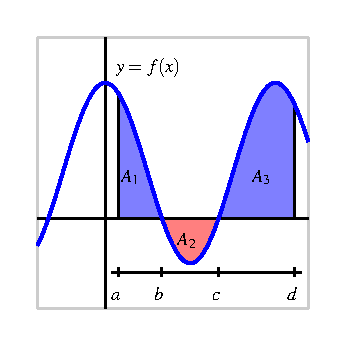
\includegraphics{figures/4_3_DefIntInterp.eps}
\caption{A continuous function $f$ on the interval $[a,d]$.} \label{F:4.3.DefIntInterp}
\end{center}
\end{figure}
For example, in the notation of the definite integral, if $f$ is the function pictured in Figure~\ref{F:4.3.DefIntInterp} and $A_1$, $A_2$, and $A_3$ are the exact areas bounded by $f$ and the $x$-axis on the respective intervals $[a,b]$, $[b,c]$, and $[c,d]$, then
$$\int_a^b f(x) \, dx = A_1, \ \int_b^c f(x) \, dx = -A_2, \ \int_c^d f(x) \, dx = A_3,$$
and
$$\int_a^d f(x) \, dx = A_1 - A_2 + A_3.$$
We can also use definite integrals to express the change in position and distance traveled by a moving object.  In the setting of a velocity function $v$ on an interval $[a,b]$, it follows from our work above and in preceding sections that the change in position, $s(b) - s(a)$, is given by
$$s(b) - s(a) = \int_a^b v(t) \, dt.$$
If the velocity function is nonnegative on $[a,b]$, then $\int_a^b v(t) \,dt$ tells us the distance the object traveled.  When velocity is sometimes negative on $[a,b],$ the areas bounded by the function on intervals where $v$ does not change sign can be found using integrals, and the sum of these values will tell us the distance the object traveled. 

If we wish to compute the value of a definite integral using the definition, we have to take the limit of a sum.  While this is possible to do in select circumstances, it is also tedious and time-consuming; moreover, computing these limits does not offer much additional insight into the meaning or interpretation of the definite integral.  Instead, in Section~\ref{S:4.4.FTC}, we will learn the Fundamental Theorem of Calculus, a result that provides a shortcut for evaluating a large class of definite integrals.  This will enable us to determine the exact net signed area bounded by a continuous function and the $x$-axis in many circumstances, including examples such as $\int_1^4 (x^2 + 1) \, dx$, which we approximated by Riemann sums in Preview Activity~\ref{PA:4.3}.

For now, our goal is to understand the meaning and properties of the definite integral, rather than how to actually compute its value using ideas in calculus.  Thus, we temporarily rely on the net signed area interpretation of the definite integral and observe that if a given curve produces regions whose areas we can compute exactly through known area formulas, we can thus compute the exact value of the integral.  
\begin{figure}[h]
\begin{center}
\scalebox{0.9}{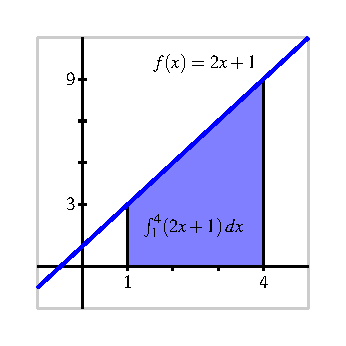
\includegraphics{figures/4_3_TrapArea.eps}}
\caption{The area bounded by $f(x)=2x+1$ and the $x$-axis on the interval $[1,4]$.} \label{F:4.3.TrapArea}
\end{center}
\end{figure}
For instance, if we wish to evaluate the definite integral  $\int_1^4 (2x+1) \, dx$, we can observe that the region bounded by this function and the $x$-axis is the trapezoid shown in Figure~\ref{F:4.3.TrapArea}, and by the known formula for the area of a trapezoid, its area is $A = \frac{1}{2}(3+9) \cdot 3 = 18$, so
$$\int_1^4 (2x+1) \, dx = 18.$$

\newpage

\begin{activity} \label{A:4.3.1}  Use known geometric formulas and the net signed area interpretation of the definite integral to evaluate each of the definite integrals below.
\ba
	\item $\ds \int_0^1 3x \, dx$
	\item $\ds \int_{-1}^4 (2-2x) \, dx$
	\item $\ds \int_{-1}^1 \sqrt{1-x^2} \, dx$
	\item $\ds \int_{-3}^4 g(x) \, dx$, where $g$ is the function pictured in Figure~\ref{F:4.3.Act1}.  Assume that each portion of $g$ is either part of a line or part of a circle.
\ea
\begin{figure}[h]
\begin{center}
\scalebox{0.9}{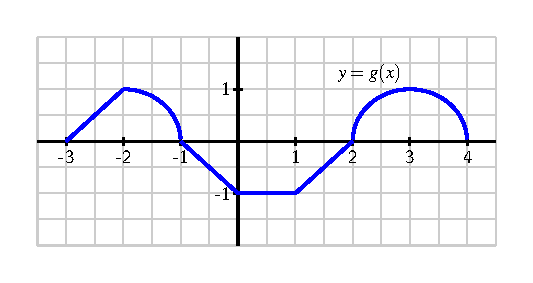
\includegraphics{figures/4_3_Act1.eps}}
\caption{A function $g$ that is piecewise defined; each piece of the function is part of a circle or part of a line.} \label{F:4.3.Act1}
\end{center}
\end{figure}
\end{activity}
\begin{smallhint}
\ba
	\item Sketch the region bounded by $y = 3x$ and the $x$-axis on $[0,1]$.
	\item Sketch the region bounded by $y = 2-2x$ and the $x$-axis on $[-1,4]$.
	\item Observe that $y = \sqrt{1-x^2}$ is the top half the circle whose equation is $x^2 + y^2 = 1$.
	\item Use known formulas for the area of a triangle, square, or circle appropriately.
\ea
\end{smallhint}
\begin{bighint}
\ba
	\item Sketch the region bounded by $y = 3x$ and the $x$-axis on $[0,1]$ and observe that it forms a familiar geometric shape.
	\item Sketch the region bounded by $y = 2-2x$ and the $x$-axis on $[-1,4]$; think carefully about the role of signed area in determining the value of the integral, and subdivide the problem by considering regions on which the curve is positive and negative.
	\item Observe that $y = \sqrt{1-x^2}$ is the top half the circle whose equation is $x^2 + y^2 = 1$.
	\item Use known formulas for the area of a triangle, square, or circle appropriately.  Keep in mind the role of signed area when dealing with the portions of the region that lie below the $x$-axis.
\ea
\end{bighint}
\begin{activitySolution}
\ba
	\item Because $y = 3x$ and the $x$-axis bound a triangle with base of length 1 and height $3$ on the interval $[0,1]$, it follows that 
	$$\ds \int_0^1 3x \, dx = \frac{1}{2} \cdot 1 \cdot 3 = \frac{3}{2}.$$
	\item For $\ds \int_{-1}^4 (2-2x) \, dx$, we first sketch the region bounded by the function, as shown below.
	\begin{center}
	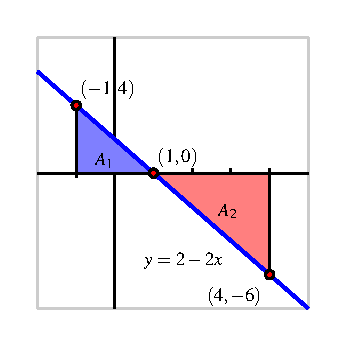
\includegraphics{figures/4_3_Act1bSoln.eps}
	\end{center}
	The line creates two triangles, one with area $A_1 = \frac{1}{2} \cdot 2 \cdot 4 = 4$ and the other with area $A_2 = \frac{1}{2} \cdot 3 \cdot 6 = 9$.  Since the latter area corresponds to a region below the $x$-axis, we associate a negative sign to it, and hence find that
	$$\int_{-1}^4 (2-2x) \, dx = A_1 - A_2 = 4 - 9 = -5.$$
	\item For $\ds \int_{-1}^1 \sqrt{1-x^2} \, dx$, we simply observe that this function is the top half of a circle of radius 1, and thus the bounded region is a semicircle of radius 1, thus having an area of $\frac{\pi}{2}$.  Therefore,
	$$\ds \int_{-1}^1 \sqrt{1-x^2} \, dx = \frac{\pi}{2}.$$
	\item Finally, for $\ds \int_{-3}^4 g(x) \, dx$, where $g$ is the function pictured in Figure~\ref{F:4.3.Act1}, we consider the function on seven consecutive subintervals of length 1.  Observe that on $[-3,-2]$, the bounded area is $\frac{1}{2}$.  On $[-2,-1]$, the area is $\frac{1}{4} \pi$.  Similarly, on the next five subintervals of length 1, the areas bounded are respectively $\frac{1}{2}$, $1$, $\frac{1}{2}$, $\frac{1}{4} \pi$, and $\frac{1}{4} \pi$.  Thus, the value of the integral is
	$$\int_{-3}^4 g(x) \, dx = \frac{1}{2} + \frac{\pi}{4} - \frac{1}{2} - 1 - \frac{1}{2} + \frac{\pi}{4} + \frac{\pi}{4} = \frac{3\pi}{4} - \frac{3}{2},$$
	which is approximately 0.8562.
\ea
\end{activitySolution}
\aftera

\subsection*{Some properties of the definite integral}

With the perspective that the definite integral of a function $f$ over an interval $[a,b]$ measures the net signed area bounded by $f$ and the $x$-axis over the interval, we naturally arrive at several different standard properties of the definite integral.  In addition, it is helpful to remember that the definite integral is defined in terms of Riemann sums that fundamentally consist of the areas of rectangles.

If we consider the definite integral $\int_a^a f(x) \, dx$ for any real number $a$, it is evident that no area is being bounded because the interval begins and ends with the same point.  Hence, 

\vspace*{5pt}
\nin \framebox{\hspace*{3 pt}
\parbox{\boxwidth}{
If $f$ is a continuous function and $a$ is a real number, then $\ds \int_a^a f(x) \,dx = 0.$
} \hspace*{3 pt}}
\vspace*{1pt}
 
\begin{figure}[h]
\begin{center}
\scalebox{0.9}{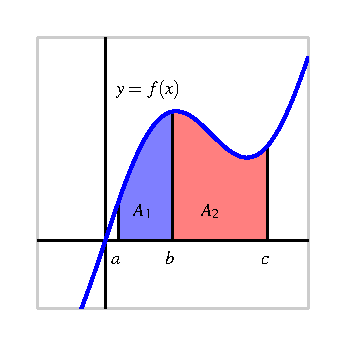
\includegraphics{figures/4_3_AdditiveProp.eps}}
\caption{The area bounded by $y=f(x)$ on the interval $[a,c]$.} \label{F:4.3.AdditiveProp}
\end{center}
\end{figure}

Next, we consider the results of subdividing a given interval. In Figure~\ref{F:4.3.AdditiveProp}, we see that
$$\int_a^b f(x) \, dx = A_1, \ \int_b^c f(x) \, dx = A_2, \ \mbox{and} \ \int_a^c f(x) \, dx = A_1 + A_2,$$ 
which is indicative of the following general rule.
  
\vspace*{5pt}
\nin \framebox{\hspace*{3 pt}
\parbox{\boxwidth}{
If $f$ is a continuous function and $a$, $b$, and $c$ are real numbers, then $$\ds \int_a^c f(x) \,dx = \int_a^b f(x) \,dx + \int_b^c f(x) \,dx.$$
} \hspace*{3 pt}}
\vspace*{1pt}

\noindent While this rule is most apparent in the situation where $a < b < c$, it in fact holds in general for any values of $a$, $b$, and $c$.  This result is connected to another property of the definite integral, which states that if we reverse the order of the limits of integration, we change the sign of the integral's value.

\vspace*{5pt}
\nin \framebox{\hspace*{3 pt}
\parbox{\boxwidth}{
If $f$ is a continuous function and $a$ and $b$ are real numbers, then 
$$\int_b^a f(x) \,dx = -\int_a^b f(x) \,dx.$$
} \hspace*{3 pt}}
\vspace*{1pt}

\noindent This result makes sense because if we integrate from $a$ to $b$, then in the defining Riemann sum $\triangle x = \frac{b-a}{n}$, while if we integrate from $b$ to $a$, $\triangle x = \frac{a-b}{n} = -\frac{b-a}{n}$, and this is the only change in the sum used to define the integral.

There are two additional properties of the definite integral that we need to understand.  Recall that when we worked with derivative rules in Chapter~\ref{C:2}, we found that both the Constant Multiple Rule and the Sum Rule held.  The Constant Multiple Rule tells us that if $f$ is a differentiable function and $k$ is a constant, then
$$\frac{d}{dx} [kf(x)] = kf'(x),$$
and the Sum Rule states that if $f$ and $g$ are differentiable functions, then
$$\frac{d}{dx}[f(x) + g(x)] = f'(x) + g'(x).$$
These rules are useful because they enable us to deal individually with the simplest parts of certain functions and take advantage of the elementary operations of addition and multiplying by a constant.  They also tell us that the process of taking the derivative respects addition and multiplying by constants in the simplest possible way.  

It turns out that similar rules hold for the definite integral.  First, let's consider the situation pictured in Figure~\ref{F:4.3.ConstMult},
\begin{figure}[h]
\begin{center}
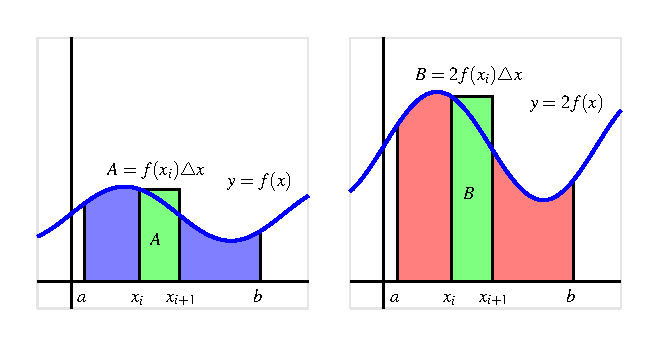
\includegraphics{figures/4_3_ConstMult.eps}
\caption{The areas bounded by $y = f(x)$ and $y = 2f(x)$ on $[a,b]$.} \label{F:4.3.ConstMult}
\end{center}
\end{figure}
where we examine the effect of multiplying a function by a factor of 2 on the area it bounds with the $x$-axis.  Because multiplying the function by 2 doubles its height at every $x$-value, we see that if we consider a typical rectangle from a Riemann sum, the difference in area comes from the changed height of the rectangle:  $f(x_i)$ for the original function, versus $2f(x_i)$ in the doubled function, in the case of left sum.  Hence, in Figure~\ref{F:4.3.ConstMult}, we see that for the pictured rectangles with areas $A$ and $B$, it follows $B = 2A$.  As this will happen in every such rectangle, regardless of the value of $n$ and the type of sum we use, we see that in the limit, the area of the red region bounded by $y = 2f(x)$ will be twice that of the area of the blue region bounded by $y = f(x)$.  As there is nothing special about the value $2$ compared to an arbitrary constant $k$, it turns out that the following general principle holds.

\vspace*{5pt}
\nin \framebox{\hspace*{3 pt}
\parbox{\boxwidth}{
{\bf Constant Multiple Rule:}\index{definite integral!constant multiple rule} If $f$ is a continuous function and $k$ is any real number then $$\ds \int_a^b k \cdot f(x) \,dx = k \int_a^b f(x) \,dx.$$
} \hspace*{3 pt}}
\vspace*{1pt}

Finally, we see a similar situation geometrically with the sum of two functions $f$ and $g$.
\begin{figure}[h]
\begin{center}
\scalebox{0.9}{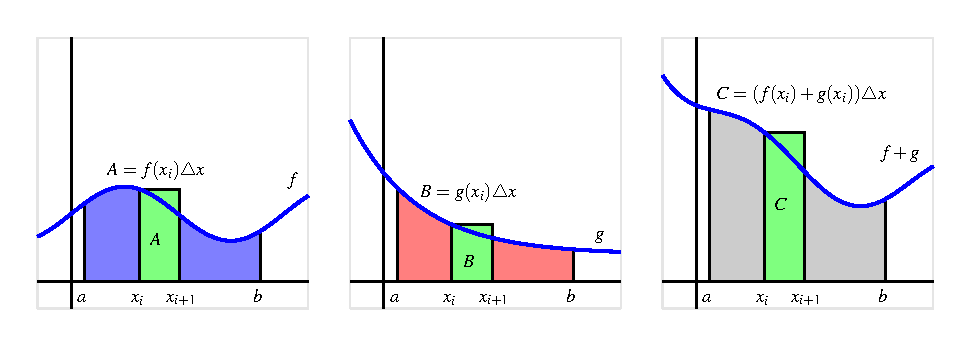
\includegraphics{figures/4_3_Sum.eps}}
\caption{The areas bounded by $y = f(x)$ and $y = g(x)$ on $[a,b]$, as well as the area bounded by $y = f(x) + g(x)$.} \label{F:4.3.Sum}
\end{center}
\end{figure}
In particular, as shown in Figure~\ref{F:4.3.Sum}, if we take the sum of two functions $f$ and $g$, at every point in the interval, the height of the function $f+g$ is given by $(f+g)(x_i) = f(x_i) + g(x_i)$, which is the sum of the individual function values of $f$ and $g$ (taken at left endpoints).  Hence, for the pictured rectangles with areas $A$, $B$, and $C$, it follows that $C = A + B$, and because this will occur for every such rectangle, in the limit the area of the gray region will be the sum of the areas of the blue and red regions.  Stated in terms of definite integrals, we have the following general rule.

\vspace*{5pt}
\nin \framebox{\hspace*{3 pt}
\parbox{\boxwidth}{
{\bf Sum Rule:}\index{definite integral!sum rule} If $f$ and $g$ are continuous functions, then $$\ds \int_a^b [f(x) + g(x)] \,dx = \int_a^b f(x) \,dx + \int_a^b g(x) \,dx.$$
} \hspace*{3 pt}}
\vspace*{1pt}

More generally, the Constant Multiple and Sum Rules can be combined to make the observation that for any continuous functions $f$ and $g$ and any constants $c$ and $k$,
$$\ds \int_a^b [c f(x) \pm k g(x)] \,dx = c \int_a^b f(x) \,dx \pm k \int_a^b g(x) \,dx.$$

\begin{activity} \label{A:4.3.2}  Suppose that the following information is known about the functions $f$, $g$, $x^2$, and $x^3$:
\begin{itemize}
	\item $\int_0^2 f(x) \, dx = -3$; $\int_2^5 f(x) \, dx = 2$
	\item $\int_0^2 g(x) \, dx = 4$; $\int_2^5 g(x) \, dx = -1$
	\item $\int_0^2 x^2 \, dx = \frac{8}{3}$; $\int_2^5 x^2 \, dx = \frac{117}{3}$
	\item $\int_0^2 x^3 \, dx = 4$; $\int_2^5 x^3 \, dx = \frac{609}{4} $
\end{itemize}
Use the provided information and the rules discussed in the preceding section to evaluate each of the following definite integrals.
\ba
	\item $\int_5^2 f(x) \, dx$
	\item $\int_0^5 g(x) \, dx$
	\item $\int_0^5 (f(x) + g(x))\, dx$
	\item $\int_2^5 (3x^2 - 4x^3) \, dx$
	\item $\int_5^0 (2x^3 - 7g(x)) \, dx$
\ea
\end{activity}
\begin{smallhint}
\ba
	\item Note that the value of $\int_2^5 f(x) \, dx$ is given.
	\item Use the values of $\int_0^2 g(x) \,dx$ and $\int_2^5 g(x) \,dx$.
	\item First find $\int_0^5 f(x) \, dx$ and $\int_0^5 g(x) \, dx$.
	\item Use the sum and constant multiple rules.
	\item First write $\int_5^0 (2x^3 - 7g(x)) \, dx = -\int_0^5 (2x^3 - 7g(x)) \, dx$.
\ea
\end{smallhint}
\begin{bighint}
\ba
	\item Note that the value of $\int_2^5 f(x) \, dx$ is given.
	\item Use the values of $\int_0^2 g(x) \,dx$ and $\int_2^5 g(x) \,dx$.
	\item First find $\int_0^5 f(x) \, dx$ and $\int_0^5 g(x) \, dx$; then use the sum rule.
	\item Use the sum and constant multiple rules.  Observe that $\int_2^5 (3x^2 - 4x^3) \, dx = 3\int_2^5 x^2 \, dx - 4\int_2^5 x^3 \, dx.$
	\item First write $\int_5^0 (2x^3 - 7g(x)) \, dx = -\int_0^5 (2x^3 - 7g(x)) \, dx$.  Then use the sum and constant multiple rules.
\ea
\end{bighint}
\begin{activitySolution}
\ba
	\item Note that the value of $\int_2^5 f(x) \, dx$ is given, and thus
	$$\int_5^2 f(x) \,dx = -\int_2^5 f(x) \, dx = -2.$$
	\item Since $\int_0^2 g(x) \,dx = 4$ and $\int_2^5 g(x) \,dx = -1$, we have
	$$\int_0^5 g(x) \,dx = \int_0^2 g(x) \,dx + \int_2^5 g(x) \,dx = 4 + (-1) = 3.$$
	\item First, using work from and similar to that in (c), we find $\int_0^5 f(x) \, dx = -3 + 2 = -1$ and $\int_0^5 g(x) \, dx = 3$, thus by the sum rule,
	$$\int_0^5 (f(x) + g(x))\, dx = \int_0^5 f(x)\, dx + \int_0^5 g(x)\, dx = -1 + 3 = 2.$$
	\item By the sum and constant multiple rules,
	$$\int_2^5 (3x^2 - 4x^3) \, dx = 3\int_2^5 x^2 \, dx - 4\int_2^5 x^3 \, dx = 3 \cdot \frac{8}{3} - 4 \frac{609}{4} = 8 - 609 = -608.$$
	\item First, we write $\int_5^0 (2x^3 - 7g(x)) \, dx = -\int_0^5 (2x^3 - 7g(x)) \, dx$.  Then, using the sum and constant multiple rules, it follows
\begin{eqnarray*}
	\int_5^0 (2x^3 - 7g(x)) \, dx & = & -\int_0^5 (2x^3 - 7g(x)) \, dx \\
					& = & -\left(2 \int_0^5 x^3 \, dx - 7 \int_0^5 g(x) \,dx \right) \\
					& = & -2 \left(\frac{8}{3} + \frac{117}{3}\right)  + 7 \left(4 +  (-1))\right) \\
					& = & -\frac{250}{3} + 21 \\
					& = & -\frac{187}{3}.
\end{eqnarray*}
\ea
\end{activitySolution}
\aftera

\subsection*{How the definite integral is connected to a function's average value} \index{average value of a function}

One of the most valuable applications of the definite integral is that it provides a way to meaningfully discuss the average value of a function, even for a function that takes on infinitely many values.  Recall that if we wish to take the average of $n$ numbers $y_1$, $y_2$, $\ldots$, $y_n$, we do so by computing
$$\mbox{Avg} = \frac{y_1 + y_2 + \cdots + y_n}{n}.$$

Since integrals arise from Riemann sums in which we add $n$ values of a function, it should not be surprising that evaluating an integral is something like averaging the output values of a function.  Consider, for instance, the right Riemann sum $R_n$ of a function $f$, which is given by
$$R_n = f(x_1) \triangle x + f(x_2) \triangle x + \cdots + f(x_n) \triangle x = (f(x_1) + f(x_2) + \cdots + f(x_n))\triangle x.$$
Since $\triangle x = \frac{b-a}{n}$, we can thus write 
\begin{equation} \label{E:RAvg}
R_n = (f(x_1) + f(x_2) + \cdots + f(x_n))\cdot \frac{b-a}{n} = (b-a) \frac{f(x_1) + f(x_2) + \cdots + f(x_n)}{n}.
\end{equation}
Here, we see that the right Riemann sum with $n$ subintervals is the length of the interval $(b-a)$ times the average of the $n$ function values found at the right endpoints.  And just as with our efforts to compute area, we see that the larger the value of $n$ we use, the more accurate our average of the values of $f$ will be.  Indeed, we will define the average value of $f$ on $[a,b]$ to be 
$$f_{\mbox{\tiny{AVG}}[a,b]} = \lim_{n \to \infty} \frac{f(x_1) + f(x_2) + \cdots + f(x_n)}{n}.$$  But we also know that for any continuous function $f$ on $[a,b]$, taking the limit of a Riemann sum leads precisely to the definite integral.  That is, $\ds \lim_{n \to \infty} R_n = \int_a^b f(x) \, dx$, and thus taking the limit as $n \to \infty$ in Equation~(\ref{E:RAvg}), we have that
\begin{equation} \label{E:RAvg2}
\int_a^b f(x) \, dx = (b-a) \cdot f_{\mbox{\tiny{AVG}}[a,b]}.
\end{equation}
Solving Equation~(\ref{E:RAvg2}) for $f_{\mbox{\tiny{AVG}}[a,b]}$, we have the following general principle.

\vspace*{5pt}
\nin \framebox{\hspace*{3 pt}
\parbox{\boxwidth}{
{\bf Average value of a function:} If $f$ is a continuous function on $[a,b]$, then its average value on $[a,b]$ is given by the formula
$$f_{\mbox{\tiny{AVG}}[a,b]} = \frac{1}{b-a} \cdot \int_a^b f(x) \, dx.$$
} \hspace*{3 pt}}
\vspace*{1pt}

Observe that Equation~(\ref{E:RAvg2}) tells us another way to interpret the definite integral:  the definite integral of a function $f$ from $a$ to $b$ is the length of the interval $(b-a)$ times the average value of the function on the interval.  In addition, Equation~(\ref{E:RAvg2}) has a natural visual interpretation when the function $f$ is nonnegative on $[a,b]$.  
\begin{figure}[h]
\begin{center}
\scalebox{0.9}{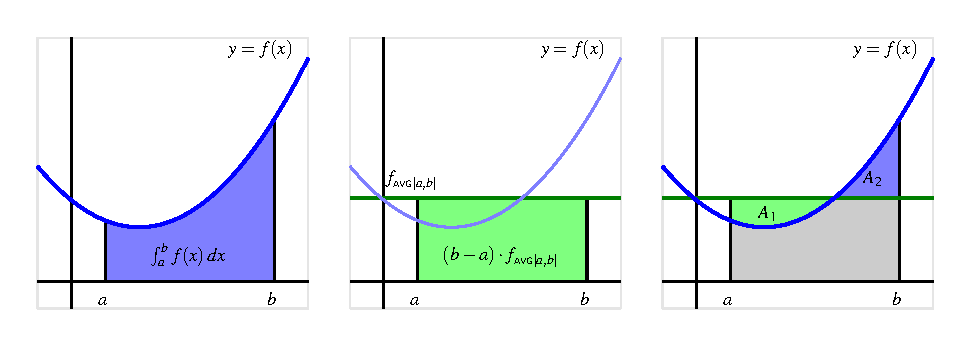
\includegraphics{figures/4_3_AvgVal.eps}}
\caption{A function $y = f(x)$, the area it bounds, and its average value on $[a,b]$.} \label{F:4.3.AvgVal}
\end{center}
\end{figure}
Consider Figure~\ref{F:4.3.AvgVal}, where we see at left the shaded region whose area is $\int_a^b f(x) \, dx$, at center the shaded rectangle whose dimensions are $(b-a)$ by $f_{\mbox{\tiny{AVG}}[a,b]}$, and at right these two figures superimposed.  Specifically, note that in dark green we show the horizontal line $y = f_{\mbox{\tiny{AVG}}[a,b]}$.  Thus, the area of the green rectangle is given by $(b-a) \cdot f_{\mbox{\tiny{AVG}}[a,b]}$, which is precisely the value of $\int_a^b f(x) \, dx$.  Said differently, the area of the blue region in the left figure is the same as that of the green rectangle in the center figure; this can also be seen by observing that the areas $A_1$ and $A_2$ in the rightmost figure appear to be equal.  Ultimately, the average value of a function enables us to construct a rectangle whose area is the same as the value of the definite integral of the function on the interval.  The java applet\footnote{David Austin, \href{http://gvsu.edu/s/5r}{\texttt{http://gvsu.edu/s/5r}}.} at \href{http://gvsu.edu/s/az}{\texttt{http://gvsu.edu/s/az}} provides an opportunity to explore how the average value of the function changes as the interval changes, through an image similar to that found in Figure~\ref{F:4.3.AvgVal}.

\begin{activity} \label{A:4.3.3}  Suppose that $v(t) = \sqrt{4-(t-2)^2}$ tells us the instantaneous velocity of a moving object on the interval $0 \le t \le 4$, where $t$ is measured in minutes and $v$ is measured in meters per minute.
\ba
	\item Sketch an accurate graph of $y = v(t)$.  What kind of curve is $y = \sqrt{4-(t-2)^2}$?
	\item Evaluate $\int_0^4 v(t) \, dt$ exactly.
	\item In terms of the physical problem of the moving object with velocity $v(t)$, what is the meaning of $\int_0^4 v(t) \, dt$?  Include units on your answer.
	\item Determine the exact average value of $v(t)$ on $[0,4]$.  Include units on your answer.
	\item Sketch a rectangle whose base is the line segment from $t=0$ to $t = 4$ on the $t$-axis such that the rectangle's area is equal to the value of $\int_0^4 v(t) \, dt$.  What is the rectangle's exact height?
	\item How can you use the average value you found in (d) to compute the total distance traveled by the moving object over $[0,4]$?
\ea
\end{activity}
\begin{smallhint}
\ba
	\item Note that $y = \sqrt{4-(t-2)^2}$ is part of the curve given by $(t-2)^2 + y^2 = 4$.
	\item What familiar shape is generated by the curve $y = v(t)$?
	\item Recall the meaning of the area bounded by a nonnegative velocity function on a given interval.
	\item From the meaning of the average value of a function, we know $v_{\mbox{\tiny{AVG}}}[a,b] = \frac{1}{b-a}  \int_a^b v(t) \, dt$.
	\item Consider a key recent figure in the text.
	\item Distance equals average rate times $\ldots$.
\ea
\end{smallhint}
\begin{bighint}
\ba
	\item Note that $y = \sqrt{4-(t-2)^2}$ is the top half of the curve given by $(t-2)^2 + y^2 = 4$, which is a familiar one.
	\item What familiar shape is generated by the curve $y = v(t)$?  What known formula for area helps?
	\item Recall the meaning of the area bounded by a nonnegative velocity function on a given interval.  See, for instance, Section~\ref{S:4.1.VelocityDistance}.
	\item From the meaning of the average value of a function, we know $v_{\mbox{\tiny{AVG}}}[a,b] = \frac{1}{b-a}  \int_a^b v(t) \, dt$.  What are $a$ and $b$ in this problem?
	\item Consider a key recent figure in the text and construct a similar drawing for the given function $v$.
	\item Distance equals average rate times time!
\ea
\end{bighint}
\begin{activitySolution}
\ba
	\item The curve $y = v(t) = \sqrt{4-(t-2)^2}$ is the top half of the circle $(t-2)^2 + y^2 = 4$, which has radius 2 and is centered at $(2,0)$.
	\item Thus, the value of $\int_0^4 v(t) \, dt$ is the area of a semicircle of radius 2, which is $\frac{1}{2} \pi (2)^2 = 2\pi$.
	\item Because the velocity $v(t)$ is always nonnegative in this problem, the meaning of $\int_0^4 v(t) \, dt = 2\pi$ is both the distance traveled and the change in position of the object on the interval $0 \le t \le \pi$.  Specifically, the object moved $2 \pi$ meters in 4 minutes.
	\item We know $v_{\mbox{\tiny{AVG}}}[a,b] = \frac{1}{b-a}  \int_a^b v(t) \, dt$, so
	$$v_{\mbox{\tiny{AVG}}}[0,4] = \frac{1}{4-0}  \int_0^4 \sqrt{4-(t-2)^2} \, dt = \frac{1}{4} 2\pi = \frac{\pi}{2},$$
	which is measured in meters per minute, since the units on ``4'' are minutes and on ``$2\pi$'' are meters.
	\item Constructing a figure similar to those shown in this section on the topic of average value of a function, we find the following, which demonstrates a rectangle having the same area as the semicircle.
	\begin{center}
	  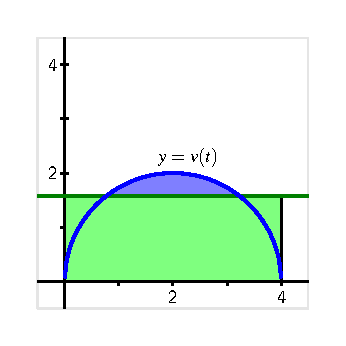
\includegraphics{figures/4_3_Act3Soln.eps}
	\end{center}
	The height of the rectangle is the average value of $v$, specifically $v_{\mbox{\tiny{AVG}}}[0,4] = \frac{\pi}{2} \approx 1.57$.
	\item Knowing that average velocity is $\frac{\pi}{2}$, it follows from the fact that distance traveled equals average rate times time (provided velocity is always nonnegative), we have
	$$D = \frac{\pi}{2} \cdot 4 = 2\pi.$$
	We see from (c) or (f) that we are simply considering the situation from two different perspectives: if we know the distance traveled, we can find average velocity, or if we know average velocity, we can find distance traveled.
\ea
\end{activitySolution}
\aftera







%\nin \framebox{\hspace*{3 pt}
%\parbox{6.25 in}{
\begin{summary}
\item Any Riemann sum of a continuous function $f$ on an interval $[a,b]$ provides an estimate of the net signed area bounded by the function and the horizontal axis on the interval.  Increasing the number of subintervals in the Riemann sum improves the accuracy of this estimate, and letting the number of subintervals increase without bound results in the values of the corresponding Riemann sums approaching the exact value of the enclosed net signed area.
\item When we take the just described limit of Riemann sums, we arrive at what we call the definite integral of $f$ over the interval $[a,b]$.  In particular, the symbol $\int_a^b f(x) \, dx$ denotes the definite integral of $f$ over $[a,b]$, and this quantity is defined by the equation
$$\int_a^b f(x) \, dx = \lim_{n \to \infty} \sum_{i=1}^{n} f(x_i^*) \triangle x,$$
where $\triangle x = \frac{b-a}{n}$, $x_i = a + i\triangle x$ (for $i = 0, \ldots, n$), and $x_i^*$ satisfies $x_{i-1} \le x_i^* \le x_i$ (for $i = 1, \ldots, n$).
\item The definite integral $\int_a^b f(x) \,dx$ measures the exact net signed area bounded by $f$ and the horizontal axis on $[a,b]$; in addition, the value of the definite integral is related to what we call the average value of the function on $[a,b]$: $f_{\mbox{\tiny{AVG}}[a,b]} = \frac{1}{b-a} \cdot \int_a^b f(x) \, dx.$  In the setting where we consider the integral of a velocity function $v$, $\int_a^b v(t) \,dt$ measures the exact change in position of the moving object on $[a,b]$; when $v$ is nonnegative, $\int_a^b v(t) \,dt$ is the object's distance traveled on $[a,b]$.  
\item The definite integral is a sophisticated sum, and thus has some of the same natural properties that finite sums have.  Perhaps most important of these is how the definite integral respects sums and constant multiples of functions, which can be summarized by the rule
$$\ds \int_a^b [c f(x) \pm k g(x)] \,dx = c \int_a^b f(x) \,dx \pm k \int_a^b g(x) \,dx$$
where $f$ and $g$ are continuous functions on $[a,b]$ and $c$ and $k$ are arbitrary constants.
\end{summary}
%} \hspace*{3 pt}}

\nin \hrulefill

\begin{exercises} 
  \item The velocity of an object moving along an axis is given by the piecewise linear function $v$ that is pictured in 
  Figure~\ref{F:4.3.Ez1}.  Assume that the object is moving to the right when its velocity is positive, and moving to the left when its velocity is negative.  Assume that the given velocity function is valid for $t = 0$ to $t = 4$.
\begin{figure}[h]
\begin{center}
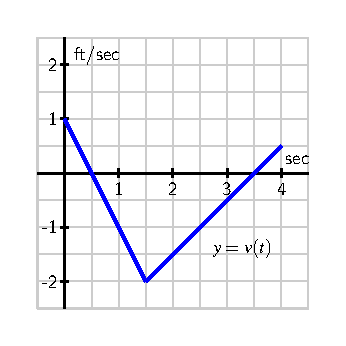
\includegraphics{figures/4_3_Ez1.eps}
\caption{The velocity function of a moving object.} \label{F:4.3.Ez1}
\end{center}
\end{figure} 
	\ba
		\item Write an expression involving definite integrals whose value is the total change in position of the object on the interval $[0,4]$.
		\item Use the provided graph of $v$ to determine the value of the total change in position on $[0,4]$.
		\item Write an expression involving definite integrals whose value is the total distance traveled by the object on $[0,4]$.  What is the exact value of the total distance traveled on $[0,4]$?
		\item What is the object's exact average velocity on $[0,4]$?
		\item Find an algebraic formula for the object's position function on $[0, 1.5]$ that satisfies $s(0) = 0$.
	\ea
	
  \item Suppose that the velocity of a moving object is given by $v(t) = t(t-1)(t-3)$, measured in feet per second, and that this function is valid for $0 \le t \le 4$.
  	\ba
		\item Write an expression involving definite integrals whose value is the total change in position of the object on the interval $[0,4]$.
		\item Use appropriate technology (such as \href{http://gvsu.edu/s/av}{\texttt{http://gvsu.edu/s/a9}}\footnote{Marc Renault, Shippensburg University.}) to compute Riemann sums to estimate the object's total change in position on $[0,4]$.  Work to ensure that your estimate is accurate to two decimal places, and explain how you know this to be the case.
		\item Write an expression involving definite integrals whose value is the total distance traveled by the object on $[0,4]$.
		\item Use appropriate technology to compute Riemann sums to estimate the object's total distance travelled on $[0,4]$.  Work to ensure that your estimate is accurate to two decimal places, and explain how you know this to be the case.
		\item What is the object's average velocity on $[0,4]$, accurate to two decimal places?
	\ea
  
        \item Consider the graphs of two functions $f$ and $g$ that are provided in Figure~\ref{F:4.3.Ez2}.  Each piece of $f$ and $g$ is either part of a straight line or part of a circle.
\begin{figure}[h]
\begin{center}
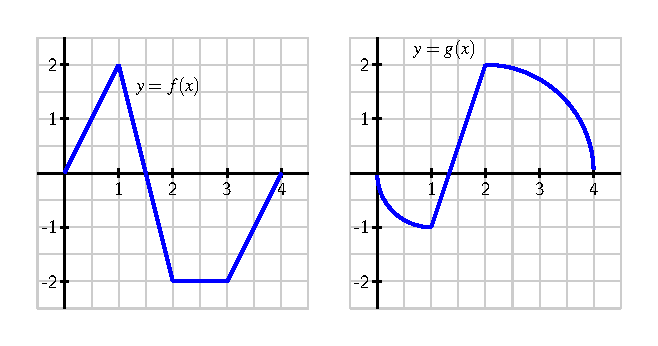
\includegraphics{figures/4_3_Ez2.eps}
\caption{Two functions $f$ and $g$.} \label{F:4.3.Ez2}
\end{center}
\end{figure} 
  \ba
  	\item Determine the exact value of $\int_0^1 [f(x) + g(x)]\,dx$.
	\item Determine the exact value of $\int_1^4 [2f(x) - 3g(x)] \, dx$.
	\item Find the exact average value of $h(x) = g(x) - f(x)$ on $[0,4]$.
	\item For what constant $c$ does the following equation hold?
	$$\int_0^4 c \, dx = \int_0^4 [f(x) + g(x)] \, dx$$
  \ea
  
    \item Let $f(x) = 3 - x^2$ and $g(x) = 2x^2$.
    \ba
    	\item On the interval $[-1,1]$, sketch a labeled graph of $y = f(x)$ and write a definite integral whose value is the exact area bounded by $y = f(x)$ on $[-1,1]$.
	\item On the interval $[-1,1]$, sketch a labeled graph of $y = g(x)$ and write a definite integral whose value is the exact area bounded by $y = g(x)$ on $[-1,1]$.
	\item Write an expression involving a difference of definite integrals whose value is the exact area that lies between $y = f(x)$ and $y = g(x)$ on $[-1,1]$.
	\item Explain why your expression in (c) has the same value as the single integral \\ $\int_{-1}^1 [f(x) - g(x)] \, dx$.
	\item Explain why, in general, if $p(x) \ge q(x)$ for all $x$ in $[a,b]$, the exact area between $y = p(x)$ and $y = q(x)$ is given by
	$$\int_a^b [p(x) - q(x)] \, dx.$$
    \ea
    

\end{exercises}
\afterexercises
 

\clearpage
